% The entire content of this work (including the source code
% for TeX files and the generated PDF documents) by 
% Hongxiang Chen (nicknamed we.taper, or just Taper) is
% licensed under a 
% Creative Commons Attribution-NonCommercial-ShareAlike 4.0 
% International License (Link to the complete license text:
% http://creativecommons.org/licenses/by-nc-sa/4.0/).
\documentclass{article}

\usepackage{float}  % For H in figures
\usepackage{amsmath} % For math
\usepackage{amssymb}
\usepackage{mathrsfs}
% Followings are for the special character: differential "d".
\newcommand*\diff{\mathop{}\!\mathrm{d}}
\newcommand*\Diff[1]{\mathop{}\!\mathrm{d^#1}}
\numberwithin{equation}{subsection} % have the enumeration go to the subsection level.
                  % See:https://en.wikibooks.org/wiki/LaTeX/Advanced_Mathematics
\usepackage{graphicx}   % need for figures
\usepackage{cite} % need for bibligraphy.
\usepackage[unicode]{hyperref}  % make every cite a link
\usepackage{CJKutf8} % For Chinese characters
\usepackage{fancyref} % For easy adding figure,equation etc in reference. Use \fref or \Fref instead of \ref
\usepackage{braket} %http://tex.stackexchange.com/questions/214728/braket-notation-in-latex

% Following is for theorems etc environments
% http://tex.stackexchange.com/questions/45817/theorem-definition-lemma-problem-numbering && https://en.wikibooks.org/wiki/LaTeX/Theorems
\usepackage{amsthm}
\newtheorem{defi}{Definition}[section]
\newtheorem{thm}{Theorem}[section]
\newtheorem{lemma}{Lemma}[section]
\newtheorem{remark}{Remark}[section]
\newtheorem{prop}{Proposition}[section]
\newtheorem{coro}{Corollary}[section]
\theoremstyle{definition}
\newtheorem{ex}{Example}[section]

% A list of nomenclatures.
\usepackage{nomencl}
\makenomenclature

\title{Miscellaneous notes for D. Huybrechts's Complex Geometry}
\date{\today}
\author{Taper}


\begin{document}


\maketitle
\abstract{
Miscellaneous notes for D. Huybrechts's book \textit{Introduction
to Complex Geometry}, include some homeworks done.
}
\tableofcontents
\section{The structure of almost complex structures on \texorpdfstring{$\mathbb{R}^{2n}$}{}}
\label{sec:The_structure_of_almost_complex_structures_on_R2n}
In exercise 1.2.1, it says that the set of all compatible almost complex
structures on a euclidean space of dimension $2n$, is two copies of $S^2$.

To show it, I tried first a straight calculation. Assuming the almost
complex structure $I= (a_{ij})$. Then we have:
\begin{figure}[H]
  \centering
  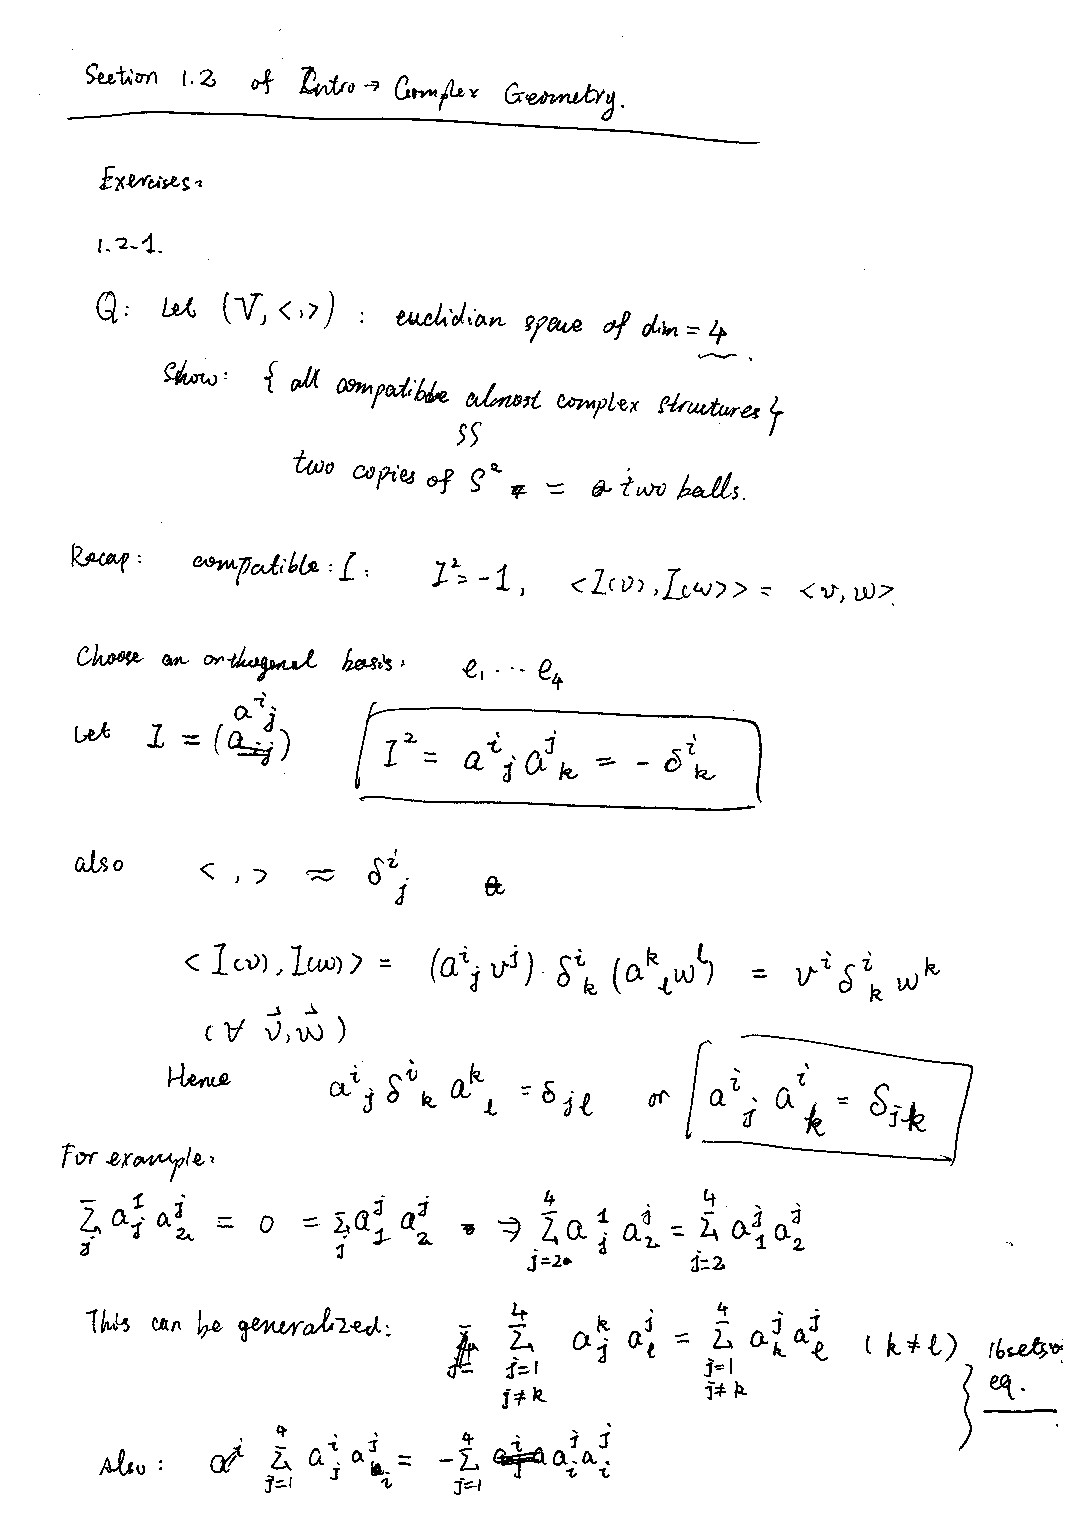
\includegraphics[scale=0.70]{pdfs/draft_20160908.pdf}
  \caption{Draft}
\end{figure}

Then I discover this too hard to work, because too many equations are
involed, and none of them could be eliminiated by other. Meanwhile, I
found a post in Math.SE about this:
\href{http://math.stackexchange.com/questions/923957/set-of-almost-complex-structures-on-mathbb-r4-as-two-disjoint-spheres}{set of almost complex structures on $\mathbb{R}^4$ as two disjoint spheres}.

To understand that post, I read this:
\href{http://math.stackexchange.com/questions/1356823/does-gln-mathbbc-inject-into-gl2n-mathbbr-for-all-n}{Does $GL(n,\mathbb{C})$ inject into $GL^+(2n, \mathbb{R})$ for all $n$?}. However, the proof inside is not perfect:
\begin{quote}
    The claim is: If $V$ is an $n$-dimensional complex vector space with underlying $2n$-dimensional real vector space $W$, then the canonical group monomorphism $\mathrm{GL}(V) \to \mathrm{GL}(W)$ lands inside $\mathrm{GL}^+(W)=\{f \in \mathrm{GL}(W) : \det(f)>0\}$.  The purpose of this abstract reformulation is that we may use operations on vector spaces in order to simplify the problem: If $V'$ is another finite-dimensional complex vector space with underlying real vector space $W'$, the diagram

    \begin{align}
      \begin{array}{ccc} 
        \mathrm{GL}(V) \times \mathrm{GL}(V') & \rightarrow & \mathrm{GL}(W) \times \mathrm{GL}(W') \\
        \downarrow & & \downarrow \\ 
        \mathrm{GL}(V \oplus V') & \rightarrow & \mathrm{GL}(W \oplus W') 
      \end{array}
    \end{align}

    commutes, and the image of $\mathrm{GL}^+(W) \times \mathrm{GL}^+(W')$  is contained in $\mathrm{GL}^+(W \oplus W')$. Therefore, if some element in $\mathrm{GL}(V \oplus V')$ lies in the image of $\mathrm{GL}(V) \times \mathrm{GL}(V')$, it suffices to consider the components. Combining this with the fact that $\mathrm{GL}(V)$ is generated by \href{https://en.wikipedia.org/wiki/Elementary_matrix}{elementary matrices} (after chosing a basis of $V$), we may reduce the whole problem to the following three types of matrices:

  - the $1 \times 1$-matrices $(\lambda)$,

  - the $2 \times 2$-matrices $\begin{pmatrix} 1 & 0 \\ \lambda & 1 \end{pmatrix}$,

  - and the $2 \times 2$-matrix $\begin{pmatrix} 0 & 1 \\ 1 & 0 \end{pmatrix}$.
   
  Write $\lambda=a+ib$ with $(a,b) \in \mathbb{R}^2 \setminus \{(0,0)\}$. Then, the complex $1 \times 1$-matrix $(\lambda)$ becomes the real $2 \times 2$-matrix $\begin{pmatrix} a & -b \\ b & a \end{pmatrix}$, which has determinant $a^2+b^2 > 0$. The complex $2 \times 2$-matrix $\begin{pmatrix} 1 & 0 \\ \lambda & 1 \end{pmatrix}$ becomes the real $4 \times 4$-matrix
  $\begin{pmatrix}
  1 & 0 & 0 & 0 \\
  0 & 1 & 0 & 0 \\
  a & -b & 1 & 0 \\
  b & a & 0 & 1 \end{pmatrix}$, which has determinant $1$. Finally, the complex $2 \times 2$-matrix  $\begin{pmatrix} 0 & 1 \\ 1 & 0 \end{pmatrix}$ becomes the real $4 \times 4$-matrix $\begin{pmatrix} 0 & 0 & 1 & 0 \\ 0 & 0 & 0 & 1\\ 1 & 0 & 0 & 0 \\ 0 & 1 & 0 & 0 \end{pmatrix}$, which has determinant $1$.

\end{quote}

This proof is not complete because, to build the proof from 
$\mathbb{R}^2$ to $\mathbb{R}^{2n}$, it requries, in his argument, that
any element in $\mathrm{GL}(V\oplus V)$ is in the image of
$\mathrm{GL}(V)\times \mathrm{GL}(V')$, which is not the case.

On the other hand, it seems that this property can be proved directly
by calculation. % TODO Start here and learn that paper.
\begin{thebibliography}{1}
  \bibitem{book} D Huybrechts's Introduction to Complex Geometry. Springer.
\end{thebibliography}
\printnomenclature
\section{License}
The entire content of this work (including the source code
for TeX files and the generated PDF documents) by 
Hongxiang Chen (nicknamed we.taper, or just Taper) is
licensed under a 
\href{http://creativecommons.org/licenses/by-nc-sa/4.0/}{Creative 
Commons Attribution-NonCommercial-ShareAlike 4.0 International 
License}. Permissions beyond the scope of this 
license may be available at \url{mailto:we.taper[at]gmail[dot]com}.
\end{document}
